\documentclass[titlepage,a4paper]{article}


\usepackage[spanish,activeacute]{babel}
%\usepackage[margin = 1in]{geometry}
\usepackage{a4wide}
\usepackage{bookmark}
\usepackage{fancyhdr}
\usepackage{graphicx}

\pagestyle{fancy} % Encabezado y pie de página
\fancyhf{}
\fancyhead[L]{TP1  - Grupo: 38}
\fancyhead[R]{Teoría de organización de datos - FIUBA}
\renewcommand{\headrulewidth}{0.4pt}
\fancyfoot[C]{\thepage}
\renewcommand{\footrulewidth}{0.4pt}





\begin{document}

	\begin{titlepage}
		\hfill
\includegraphics[width=6cm]{logofiuba.jpg}
		\center
		\vfill
		\vfill
		\begin{center}
			\begin{Huge}\textbf{Trabajo Práctico Nº 1}\end{Huge}\\
			\vfill
			\begin{huge}Análisis Exploratorio\end{huge}\\
			\vfill
			\begin{Large} Teoría de Organización de Datos\end{Large}\\

			\textbf{Nombre grupo:} "The data inception" \\
			\textbf{Nº grupo: 38}\\
				Todo el trabajo realizado puede encontrarse en el siguiente repositorio de github:\textit{ https://github.com/sebalogue/tp1-datos.git. }
	
			\vfill
			\begin{tabular}{|c|c|c|}
				\hline
				participantes & nº padrón & mail \\ \hline
				LOIS,Lucas Edgardo &[COMPLETAR] &  [COMPLETAR] \\ \hline		
				LOGUERCIO, Sebastian Ismael &[COMPLETAR] &  [COMPLETAR] \\ \hline
				MARIANI, Santiago Tomás &[COMPLETAR] &  [COMPLETAR] \\ \hline
				MARIJUAN, Magalí & 100070 & maguimar001@gmail.com\\ \hline
				
			\end{tabular}
			\vfill
			\vfill
			\vfill
			\vfill
			\vfill
			\vfill
		\end{center}
	
	\end{titlepage}

	\tableofcontents
	\newpage
	
	\section{Introducción:}
	Este trabajo práctico consitía en realizar un análisis sobre un conjunto de eventos de web analytics de usuarios que visitaron www.trocafone.com, su plataforma de ecommerce de Brasil.
	
	Para realizar dicho trabajo utilizamos el lenguaje de programación \textit{Python}. Para el análisis de datos usamos la librería \textit{Pandas} y para la realización de gráficos utilizamos la librerías \textit{Matplotlib }y \textit{Sns}. Por otro lado, trabajamos usando el sistema de control de versiones \textit{GIT}	
	
	En nuestra primera experiencia realizando un análisis exploratorio, nos dimos cuenta que una buena abstracción para realizar el trabajo práctico era: \textbf{preguntandole al dataset}. Es decir que en nuestro modelo siempre hacíamos preguntas que luego intentabamos responder con los datos que podíamos obtener del dataset. 
	
	\section{Análisis Preliminar}
	En un primer análisis intentamos entender cómo estaba compuesto el data set. Es decir, cuáles son los eventos que los componenen, cómo interactúan como un conjunto y cuáles son las características propias de cada evento. 
	\subsection{Eventos}
	El dataset contenia los siguiente eventos: 
	\begin{itemize}
	\item Viewed product: El usuario visita una página de producto.
	\item Brand listing: El usuario visita un listado específico de una marca viendo un conjunto de productos.
	\item Visited site: El usuario ingresa al sitio a una determinada url.
	\item Ad campaign hit:  El usuario ingresa al sitio mediante una campana de marketing online.
	\item Generic listing:  El usuario visita la homepage.
	\item Serched products:  El usuario realiza una búsqueda de productos en la interfaz de búsqueda del site.
	\item Search engine hit: El usuario ingresa al sitio mediante un motor de búsqueda web.
	\item Checkout: El usuario ingresa al checkout de compra de un producto.
	\item Staticpage: El usuario visita una página.
	\item Conversion: El usuario realiza una conversión, comprando un producto.
	\item Lead: El usuario se registra para recibir una notificación de disponibilidad de stock, para un producto que no se encontraba disponible en ese momento.
	
	\newpage
	La cantidad total de eventos fue: 	1011288. Ellos se distribuyeron de la siguiente manera:
	\end{itemize}
	\begin{center}
	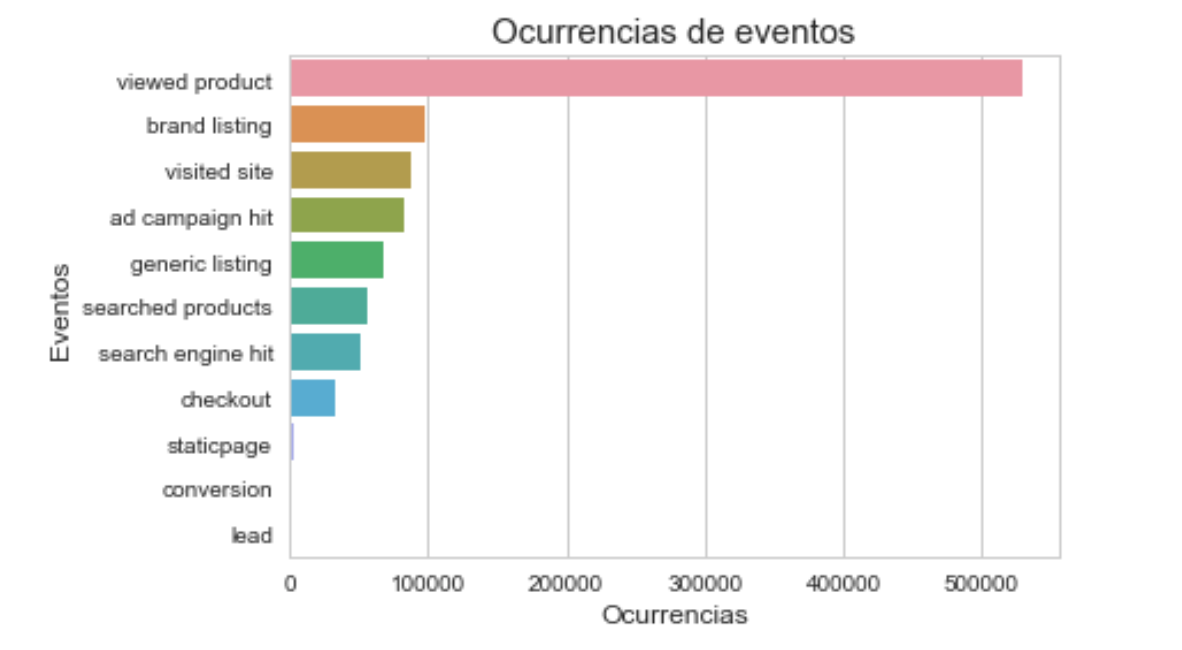
\includegraphics[width=10cm]{ocurrencia_eventos.jpg}\\
	\textbf{Figura 1:}  \textit{En este gráfico se puede ver los eventos y la cantidad de apariciones que tuvieron en el dataset. }
	\end{center}
	Nos dimos cuenta que no todos los campos del data set eran relevantes para todos los eventos, por lo tanto, mediante un análisis de elementos nulos llegamos a las siguientes conclusiones: 
	\begin{itemize}
		\item Todos los eventos tiene información temporal y sobre la persona que realizó dicho evento. 
		\item Para el evento \textbf{viewed product} sus campos obligatorios son: timestamp , sku , model, condition, storage, color.
		\item Para el evento \textbf{brand listing} su campo obligatorio es: skus. 
		\item Para el evento \textbf{visited site} sus campos obligatorios son: channel, new vs returning, city, region, country, device tipe , screen resolution, operating system version y browser version.
		\item Para el evento \textbf{ad campaing hit} sus campos obligatorios son: url  y campaing source.
		\item Para el evento \textbf{generic listing} su campo obligatorios es: skus.
		\item Para el evento  \textbf{serched product } sus campos obligatorios son: skus y search term.
		\item Para el evento \textbf{serched engine} su campo obligatorio es: search engine
		\item Para el evento \textbf{checked out}  sus campos obligatorios son: sku, color, storage, model y condition 
		\item Para el evento \textbf{static page}  sus campo obligatorio es: satatic page
		\item Para le evento \textbf{conversion} sus campos obligatorios son:  sku, model, color , condition y storage
		\item Para el evento \textbf{lead} su campo obligatorio es: model

	\end{itemize}	
	
	Como todos los eventos tenían información temporal. Decidimos análizar la cantidad de eventos que se realizan por hora del día y el resultado fue:
	\begin{center}
	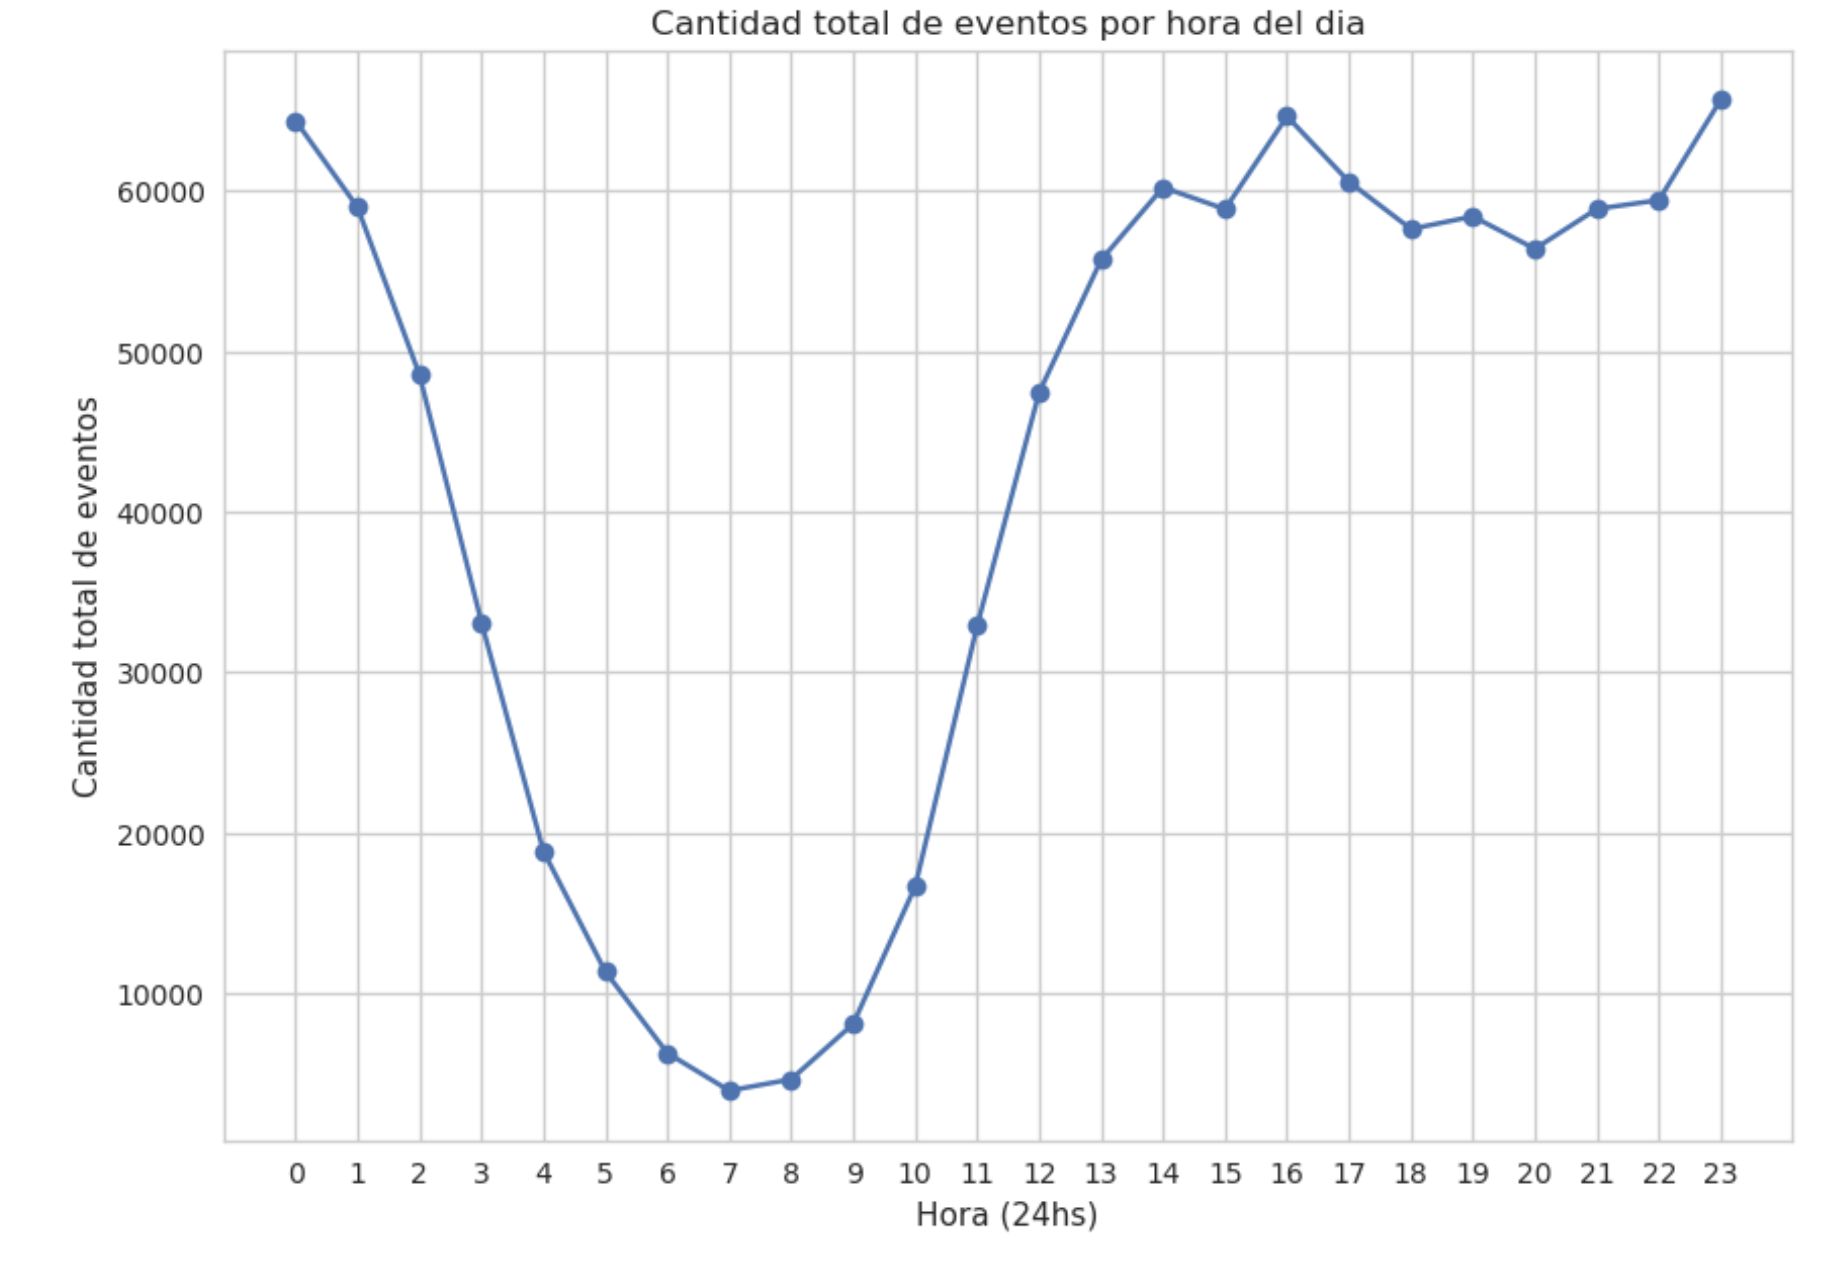
\includegraphics[width=10cm]{cantidadDeEventosPorHoraDelDia.jpg}\\
	\textbf{Figura 2:}  \textit{En este gráfico se puede ver los eventos y su distribución a lo largo del día. }
	\end{center}
	Por lo tanto, la mayoría de los eventos se efectúan entre las 10 am y 2 am. 
	
	\subsection{Viewed product}
	La primera columna que decidimos analizar fue model. De ella obtuvimos los 15 celulares más vistos, ellos fueron:
	\begin{center}
	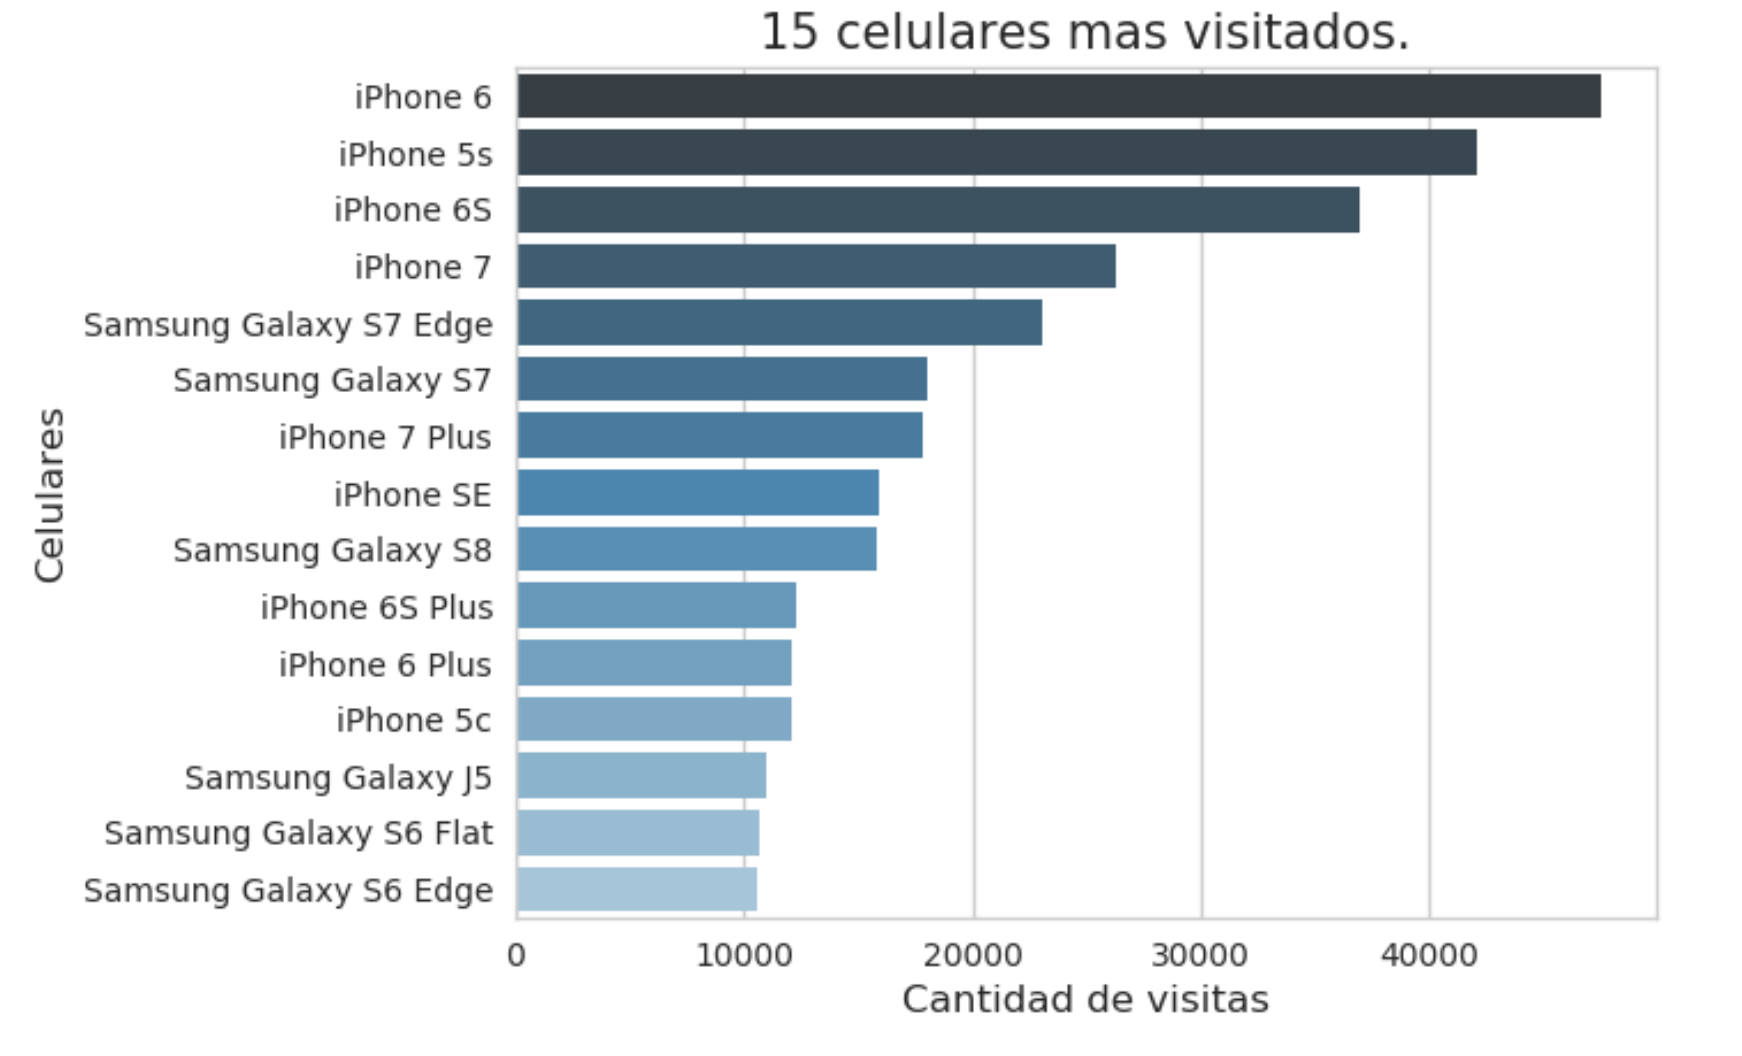
\includegraphics[width=10cm]{15celularesMasVisitados.jpg}\\
	\textbf{Figura 3:}  \textit{En este gráfico se pueden ver los 15 celulares más vistos.  }
	\end{center}
	 Sobre las características de esos modelos primero analizamos el color de los productos vistos y concluímos que: 
	 El 50\% de de los usuarios concentró su elección en los siguientes colores:
	 \begin{itemize}
	 \item El 23\% de los productos son negro.
	\item El 20\% de los productos son dorados.
	\item El 11\% de los productos son gris espacial.
	\end{itemize}	  
	Luego analizamos el almacenamiento de los productos y concluímos que:
	\begin{itemize}
	\item El 33\% visita productos con almacenamiento de 16 GB.
    \item El 32\% visita productos con almacenamiento de 32 GB.
    \item El 17\% visita productos con almacenamiento de 64 GB.
    \item El 6\% visita productos con almacenamiento de 8 GB.
	\end{itemize}
	Por último analizamos las condiciones d elos productos vistos y concluímos que:
	\begin{itemize}
	\item El 0,02 porciento de los productos que visita el usuario son nuevos.    
    \item El 2\% de los productos que tienen identificador de huella digital. 
    \item El 42\% de los productos son de calidad buena.
    \item El 27\% de los productos son de calidad excelente .
    \item El 27\% de los productos son de calidad muy buena.
	\end{itemize}
	Realizamos un análisis temporal sobre el evento y obtuvimos que:
	
	\begin{center}
	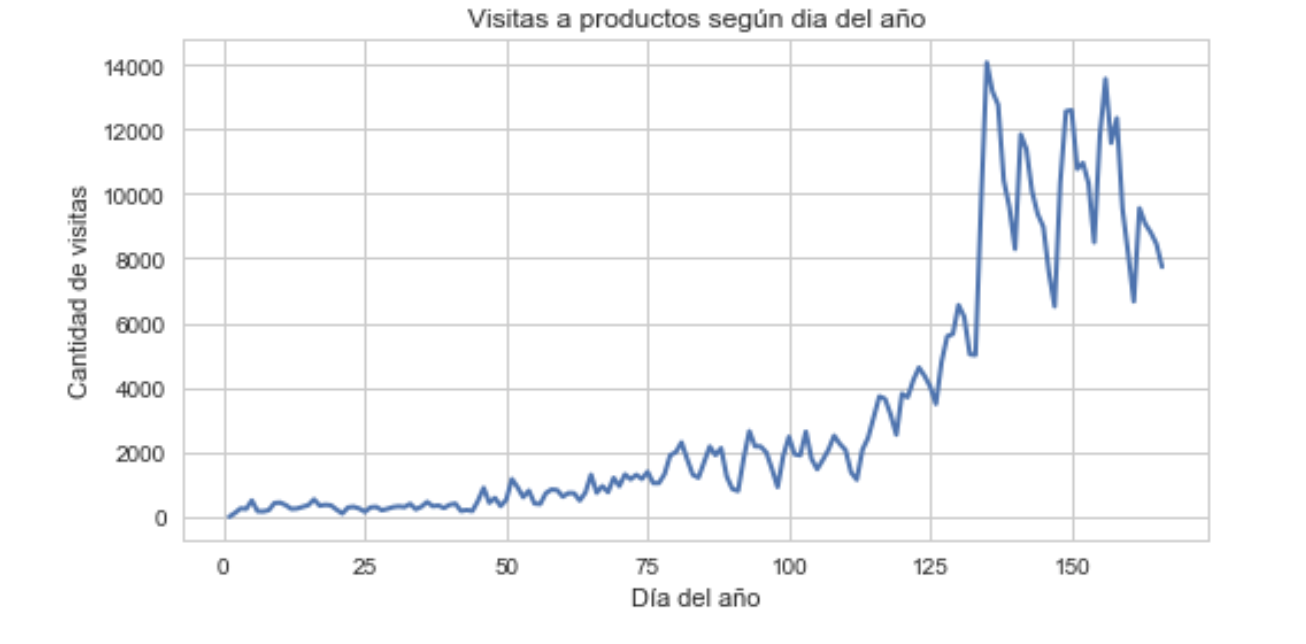
\includegraphics[width=10cm]{VisitasAProductosSegunDiaAnio.jpg}\\
	\textbf{Figura 4:}  \textit{En este gráfico se puede ver como fueron las visitas según los días del año  }
	\end{center}

	\begin{center}
	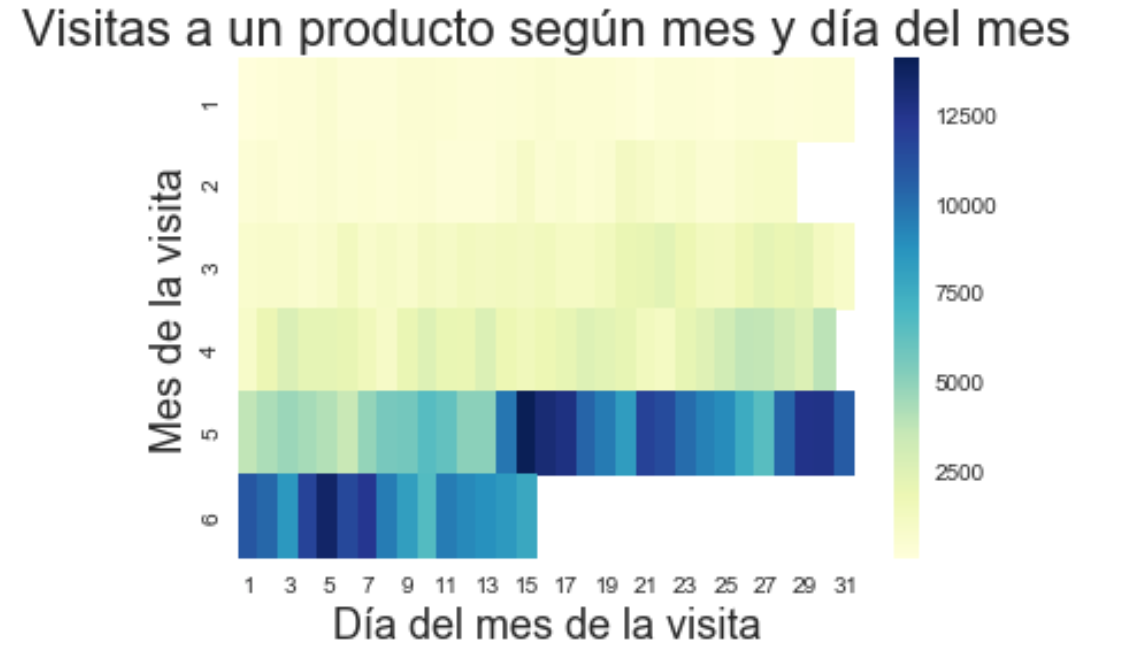
\includegraphics[width=10cm]{visitasSegunmesDiaMes.jpg}\\
	\textbf{Figura 5:}  \textit{En este gráfico se pueden ver como fueron las visitas a un producto según mes y el día del mes.   }
	
	\end{center}
	\begin{center}
	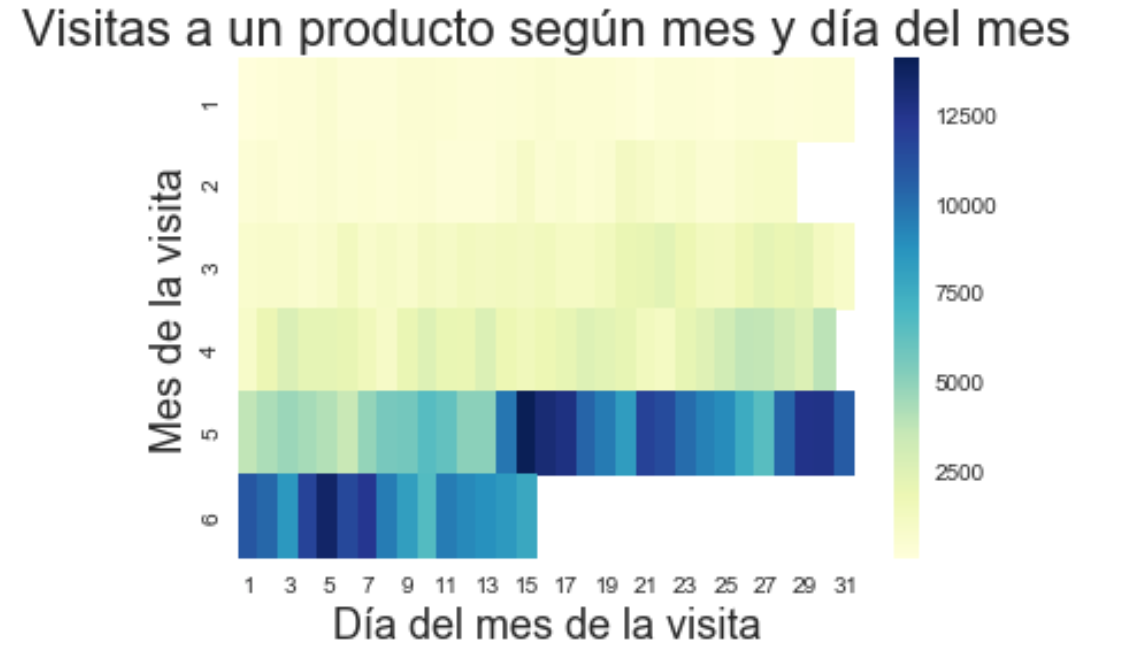
\includegraphics[width=10cm]{visitasSegunmesDiaSemana.jpg}\\
	\textbf{Figura 6:}  \textit{En este gráfico se pueden ver como fueron las visitas según el mes y el día de la semana.    }
	\end{center}
	

	
	
	
	
\end{document}